% !TEX encoding = UTF-8 Unicode

\documentclass{report}

\usepackage{amsmath,amssymb, amsfonts, amsthm, titling, url, array}
\usepackage[hangul]{kotex}
\usepackage{kotex-logo}

\usepackage{iftex}
\ifPDFTeX
  \usepackage{dhucs-nanumfont}
\else\ifXeTeX
  \setmainhangulfont[Ligatures=TeX]{HCR Batang LVT}
  \setsanshangulfont[Ligatures=TeX]{HCR Dotum LVT}
\else\ifLuaTeX
  \setmainhangulfont[Ligatures=TeX]{HCR Batang LVT}
  \setsanshangulfont[Ligatures=TeX]{HCR Dotum LVT}
\fi\fi\fi
\usepackage{tikz}
\usepackage{tcolorbox}

\setlength{\parindent}{0.4em}
\setlength{\parskip}{0.5em}

\theoremstyle{plain}
\newtheorem{thm}{Theorem}[section]
\newtheorem{lem}[thm]{Lemma}
\newtheorem{prop}[thm]{Proposition}
\newtheorem*{cor}{Corollary}

\theoremstyle{definition}
\newtheorem{defn}{Definition}[section]
\newtheorem{conj}{Conjecture}[section]
\newtheorem{exmp}{Example}[section]

\theoremstyle{remark}
\newtheorem*{rem}{Remark}
\newtheorem*{note}{Note}


\begin{document}

\title{Distributed Algorithms}
\author{Nancy Lynch}
\date{\today}

\maketitle

\newpage
\tableofcontents
\newpage
\pagenumbering{arabic}

\chapter{필사}

\section{공부하기}

분산 처리는 게임 서버에서 가장 중요한 기반 기술 중 하나이지만 
제대로 이해하고 활용해서 단단한 토대를 구성하는 노력이 부족했다. 

이제 Nancy Linch의 고전적인 대학원 강의 자료를 필사하면서 
중요한 개념들을 이해하고 개발에 활용하고자 한다.

\subsection{\LaTeX 으로 필사하기}

인터넷에서 구한 원본이 \TeX으로 작성되었고 언젠가 한번은 마스터 해야겠기에 
이번 필사를 \LaTeX으로 진행한다. 

문서 작성에 이만한 도구가 없기도 해서 이번에 제대로 같이 배우고자 한다. 

\subsubsection{\LaTeX 익히기}

한글 article 템플릿 문서에서 시작한다. HCR 기본 폰트가 가독성도 높고 
기본 구성도 괜찮은 편이다. 예쁜 문서가 되려면 할 일이 많겠으나 
별첨에 \LaTeX 공부한 내용을 정리하면서 진행한다. 

\subsection{끝까지 하기}

대학원 강의라 생각보다 어려운 경우가 많고 활용을 바로 하기도 쉽지 않을 터라 
중간 중간 좌절할 수 있겠지만 끝까지 진행한다. 

기본은 필사이다. 

\chapter{Lecture 1}

\section{Introduction to the Course}

\subsection{The Subject Matter}

"Distributed Algorithms" including a wide range of parallel algorithms,
which can be classified by a variety of attributes: 

\begin{itemize}
    \item Interprocess Communication (IPC) method: shared memory, message passing, dataflow.
    \item Timing Model: synchronous, asynchronous, partially synchronous
    \item Failure Model: reliable system, faulty links, faulty processors. 
    \item Problems addressed: resource allocation, communication, agreement, database concurrency control, deadlock detection, and many more. 
\end{itemize}

Some of the major intended application areas of distributed algorithms are: 
\begin{itemize}
    \item communication systems
    \item shared-memory multiprocessor computation 
    \item distributed operating systems
    \item distributed database systems, 
    \item digital circuits, and 
    \item real-time process-control systems. 
\end{itemize}

The algorithms to be studied in this course are distinguished by having a higher
degree of uncertainty, and more independence of activities: Some of the types of
uncertainty that will consider are: 
\begin{itemize}
    \item unknown number of processors, 
    \item unknown shape of network, 
    \item independent inputs at different locations, 
    \item serveral programs executing at once, starting at different times, going at different speeds, 
    \item nondeterministic processors
    \item ucertain message delivery times, 
    \item unknown message ordering
    \item failures: procesor (stopping, transient omission, Byzantine); link (message loss, duplication, reodering)
\end{itemize}

Because of all this uncertainty, no component of a distributed system "knows" the 
entire system state. 

Distributed algorithms can be extremely complex, at least in their details, 
and can be quite difficult to understand. Even though the actual code may be
short, the fact that many processors are executing the code in parallel, 
with steps interleaved in some undetermined way, implies that ther can be 
prohibitively many different executions, even for the same inputs. This implies
that it is nearly impossible to understand everything about the executions of 
distributed algorithms. 

Therefore, instead of trying to understand all the details of the execution, 
one tends to assert certain properties of the execution, and just understand
and prove these properties.

\subsubsection{Style}

The general flavor of the work to be studied is as follows:
\begin{itemize}
    \item Identify problems of major significance in (proactical) distributed 
    computing and define abstract versions of the problems for mathematical 
    study. 
    \item Give precise problem statements.
    \item Describe algorithms precisely. 
    \item Prove rigorously that the algorithms solve the problems. 
    \item Analyze the complexity of the algorithms. 
    \item Prove corresponding impossibility results. 
\end{itemize}

Note the emphasis on right; A rigorous approach seems necessary to be sure that
the problems are meaningful, the algorithms are correct, the impossibility results
are true and meaningful, and the interfaces are sufficiently well-defined to 
allow system building. 

...

So, rigor is a goal to be striven for, rather than one that we will achiee entirely
in this course.

\subsubsection{Overview of the Course}

Timing models: 
\begin{itemize}
    \item synchronous: 
    \item asynchronous: 
    \item partially synchronous (timing based):
\end{itemize}

IPC mechanism: shared memory vs. message-passing. 
And finally, each model and problem can be considered with various failure 
assumptions. 

\noindent \textbf{Models and Proof Methods.} The basic models used are 
\textit{automata-theoretic}, 
starting with a basic state-machine model with little structure. 
\textit{Invariant assertions} are often proved about automaton states, by induction. 
Another model is the I/O automaton model for \textit{reactive systems}, i.e., 
systems that interact with an external environment in an ongoing fashion. 
This model can model systems based on shared variables, but is more appropriate
for message-passing systems. One of the key features of this model is that it 
has good \textit{compositionality} properties, e.g., that the correctness of a 
compound automaton can be proved using the correctness of its components. 
\textit{Temportal logic} is an example of a special set of methods (language, logic)
mainly designed for proving \textit{liveness} properties (e.g., something
eventually happens). \textit{Timed models} are mainly newer research work. Typically
, there are specially-tailored models for talking about timing-based systems 
- e.g., those whose components have access to system clocks, can use timeouts, etc. 
\textit{Algebraic methods} are an important research subarea (but we will not have
time for this). The algebraic methods describe concurent processes and systems 
using algebraic expressions, the use equations involving these expressions to 
prove equialences and implementation relationships amonth the processes. 

\noindent \textbf{Synchronous Message-Passing.} We have the processors at the nodes of a graph
G, communicating with their neighbors via messages in the edges. We start with 
a simple toy example, involving \textit{ring computation}. ...... 
For example, we shall show upper and lower bounds for the time and the amount of
communication (i.e., number of messages) required. 
Then we turn to the problem of \textit{reaching consensus}. The uncertainty 
here stems from not only from different initial opinions, but also from 
\textit{processor failures}. We consider failures of different types: stopping, 
ommision, where messages may be lost en route; and byzantine, where a faulty 
processor is completely unrestricted. 

\noindent \textbf{Asynchronous Shared Memory.} After "warming up" with synchronous
algorithms (in which there is only a little uncertainty), we move into the more
characteristic (and possibly more interesting) part of the course, on 
\textit{asynchronous} algorithms. 

The first problem we deal with is \textit{mutual exclusion}. This is one of the 
fundamental (and historically first) problems in this area, and consequently, 
much work has been dedicated to exploring it. ... 
Many important concepts for this field will be illustrated in this context, 
including progress, fairness, fault-tolerance, and time analysis for asynchronous
algorithms. We shall see upper bounds on the amount of shared memory, corresponding
lower bounds, and impossibility results. We shall also discuss generalizations 
of mutual exclusion to more general resource allocation problems. For example, 
we will consider the \textit{Dining Philosophers} problem - a prototypical 
resource allocation problem. 

Next, we shall study the concept of \textit{atomic registers}: so far, we 
have been assuming indivisible access to shared memory. But how can one 
implement this on simpler architectures? An interesting new property that appears
here is \textit{wait-freeness}, which means that any operation on the register
must complete regardless of the failure of other concurrent operations. 

An \textit{atomic snapshot} is a convenient primitive for share read-write memory. 
Roughly speaking, the objective is to take an instantaneous snapshot of all memory 
locations at once. 

A \textit{concurrent timestamp system} is another nice primitive. This is a system
that issues, upon request, timestamps that can be used by programs to establish 
a consistent order among their operations. The twist here is how to implement 
such systems with bounded memory. A concurrent timestamp system can be used to 
build more powerful forms of shared memory, such as multi-writer multi-reader memory. 

We shall also reconsider the \textit{concensus} problem in the asynchronous Shared
memory model, and prove the interesting fact it is impossible to solve in this setting. 

\noindent \textbf{Asynchronous Message-Passing Systems.} This section deals with 
algorithms that operate in async networks. Again, the system is modeled as a graph
with processors at nodes, and communication links are represented by the edges, 
but now the system does not operate in rounds. In particular, messages can arrive
at arbitrary times and the processors can take steps at arbitrary speeds. One might
say that we now have "looser coupling" of the components of the system: we have
more independence and uncertainty. 

\textit{Computing in static graphs.} Graph가 고정되고 시작 시 입력이 전달되고 하나의 
결과만 출력하는 고정된 그래프 구성. 

\textit{Network Synchronization.} At this point, we could plunge into a study the 
many special-purpose algorithms designed expressly for asynchronous distributed
networks. But instead, we shall first try to impose some structure on such algorithms
by considering "algorithm transformations" that can be used to run algorithms 
designed for a simpler computation model on a complex asynchronous network. 

The first example here arises in the very important paper by Lamport, where he 
shows a simple method of assigning consistent \textit{logical times} to events
in a distributed network. This can be used to allow an asynchronous network to 
simulate one in which the nodes have access to perfectly synchronized real-time
clocks. The second example is Awerbuch's \textit{synchronizer}, which allows
an asynchronous network to simulate the lock-step synchronous networks discussed
in the first part of the course, and to do so efficiently. 

\textit{Detection of stable properties} refers to a class of problems with a similar 
flavor and a common solution. Suppose that there is a separate algorithm running, 
and we want to design another algorithm to "monitor" the first. To monitors here
mean, for instance, to detect when it terminates or deadlocks, or to take  
"consistent snapshot" of its state.

\textit{Dtalink} protocols involve the implementation of a reliable communication link 
in terms of unrealible underlying channles. We shall see the basic Alternating Bit 
Protocol ( the standard case study for concurrent algorithm verification papers).

\textit{Special-Purpse Network Building Blocks.} Major examples are the protocols
of broadcast-convergecast, reset, end-to-end. 

\textit{Self-stabilization.} Informally, a protocol is said to be self-stabilizing 
if its specification does not require a certain "initial configuratin" to be imposed
on the system to ensure correct behavior of the protocol. 

\noindent \textbf{Timing-based Systesm.} These systesm lie between synchronous and 
asynchronous, so they have somewhat less uncertainty than the latter. 
In these systems, processors have some knowledge of time, for example, access to 
real time, or approximate real time, or some timeout facility. 

\subsection{Synchronous Network Algorithms}

Nodes organized into a directed graph \\ 
$G=(V, E)$ : directed graph. size is $n=|V|$.  \\
$M$ : Message alphabet. $null$ denote the absence of a message. 

Each node $i \subset V $ has: 
\begin{description}
  \item $states(i)$ : a set of states 
  \item $start(i)$  : a subset of $states(i)$ 
  \item $msgs(i)$   : mapping $states(i) \times out-nbrs(i)$ 
  to elements of $M$ or $null$
  \item $trans(i)$  : mapping $states(i)$ and a vector of messages in 
  $M \cap {null}$, one per in-neighbor of $i$, to $states(i)$
\end{description}

\begin{tcolorbox}[title=노트]
$states, start, msgs, trans$ are all denoted with a function of a node index $i$. 
$msgs(i)$ is a function $ msg: M\cup{null} \times out-nbrs(i) \rightarrow states(i)$.

방향을 갖는 그래프로 $in-nbrs(i)$ 와 $out-nbrs(i)$ 는 단방향, 양방향에 모두 적용될 수 있다. 
$|V|$는 그냥 $n$으로 많이 표시되므로 문맥에서 잘 찾아야 한다. 
\end{tcolorbox}

Execution begins with all the nodes in some start states, and all channels empty. Then
the nodes, in lock step, repeatedly execute the following procedure called round.
\begin{enumerate}
    \item Apply message generation function to generate messages for out neighbors
    \item Put them in the channels.
    \item Apply transition function to the incoming messages and the state to get 
the new state.
\end{enumerate}

\begin{tcolorbox}[title=노트]
channel이 노드의 edge에 $M$의 알파벳을 보내고 받는 기능을 부여했다.\\
lock step을 어떻게 달성할 지에 대한 언급 없이 그냥 가능하다고 가정했다. 
그 자체로 매우 중요한 가정이다. 
\end{tcolorbox}

\subsubsection{Problem Example: Leader Election in a Ring}

Graph that is a ring, plus an extra dummy node. The ring is unidirectional 
(messages can be sent only clockwise). The ring is of arbitrary size, 
unknown to the processors (i.e., size information is not built into their states). 

The requirement is that eventually, exactly one process outputs a $leader$ 
message on its dummy outgoing channel. 

\begin{prop}[Impossibility under Symmetry]
If all the nodes in the ring have identical state sets, start states, message functions
and transition functions, then they do not solve the leader election problem for 
$n > 1$.
\end{prop}

\begin{proof}
It is straightforward to verify, by \textbf{induction on the number of rounds}, 
that all the processors are in identical states, after any number of rounds.

\end{proof}


\chapter{Appendix}
\section{Appendix 1. \LaTeX 익히기}

\subsection{Drawing Diagrams}

빠르게 그릴 수 있다면 직관적인 이해를 높일 수 있다. 

\subsubsection{기본 기능}

\begin{verbatim}
\setlength{\unitlength}{0.20mm}
\begin{picture}(400,250)
\put(75,10){\line(1,0){130}}
\put(75,50){\line(1,0){130}}
\put(75,200){\line(1,0){130}}
\put(120,200){\vector(0,-1){150}}
\put(190,200){\vector(0,-1){190}}
\put(97,120){$\alpha$}
\put(170,120){$\beta$}
\put(220,195){upper state}
\put(220,45){lower state 1}
\put(220,5){lower state 2}
\end{picture}
\end{verbatim}

아래 그림을 만든다. 좌표계와 위치를 지정하고 line / vector / circle / oval을 
사용한다. 추가 오브젝트들도 있을 것이다. 

\setlength{\unitlength}{0.20mm}
\begin{picture}(400,250)
\put(75,10){\line(1,0){130}}
\put(75,50){\line(1,0){130}}
\put(75,200){\line(1,0){130}}
\put(120,200){\vector(0,-1){150}}
\put(190,200){\vector(0,-1){190}}
\put(97,120){$\alpha$}
\put(170,120){$\beta$}
\put(220,195){upper state}
\put(220,45){lower state 1}
\put(220,5){lower state 2}
\end{picture}

\subsubsection{TikZ package}

tikz와 pgf는 위대한 라이브러리이다. 다른 위대함이 텍 안에 많지만 놀랍다. 

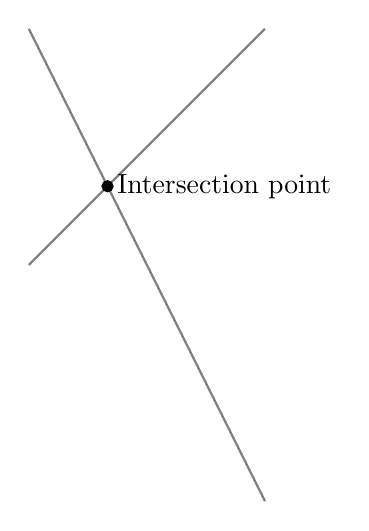
\begin{tikzpicture}
\draw[gray, thick] (-1,2) -- (2,-4);
\draw[gray, thick] (-1,-1) -- (2,2);
\filldraw[black] (0,0) circle (2pt) node[anchor=west] {Intersection point};
\end{tikzpicture}

완전한 매뉴얼이 상세한 튜토리얼을 포함해서 아래에 있다.  

http://mirror.utexas.edu/ctan/graphics/pgf/base/doc/pgfmanual.pdf


% latex is still hard to master. 



\end{document}
